\documentclass[11pt,reqno]{amsart}
\usepackage[T1]{fontenc}
\usepackage{lmodern}
\usepackage[a4paper,margin=25mm]{geometry}
\usepackage{mathtools,amssymb,amsthm}
\usepackage{microtype}
\usepackage{graphicx,booktabs,array}
\usepackage{float,placeins}
\usepackage{xcolor}
\usepackage[numbers,sort&compress]{natbib}
\usepackage{xurl}
\usepackage{tikz}
\usetikzlibrary{arrows.meta,calc,graphs}
\renewcommand{\topfraction}{0.95}
\renewcommand{\textfraction}{0.05}
\renewcommand{\floatpagefraction}{0.75}
\setcounter{topnumber}{3}
\usepackage[hidelinks]{hyperref}
\hypersetup{pdftitle={Selecting LLM workflow graphs and reasoning settings under service constraints},pdfauthor={Emmett Miller}}
\newtheorem{theorem}{Theorem}[section]
\newtheorem{lemma}[theorem]{Lemma}
\newtheorem{proposition}[theorem]{Proposition}
\newtheorem{corollary}[theorem]{Corollary}
\theoremstyle{definition}
\newtheorem{definition}[theorem]{Definition}
\newtheorem{assumption}[theorem]{Assumption}
\newtheorem{example}[theorem]{Example}
\theoremstyle{remark}
\newtheorem{remark}[theorem]{Remark}
\newcommand{\E}{\mathbb E}
\newcommand{\Prob}{\mathbb P}
\newcommand{\ind}{\mathbf 1}
\newcommand{\R}{\mathbb R}
\newcommand{\W}{\mathcal W}
\newcommand{\M}{\mathcal M}
\DeclareMathOperator{\softmax}{softmax}
\DeclareMathOperator{\argmin}{argmin}
\title[Selecting LLM graphs and settings]{Selecting LLM workflow graphs and reasoning settings under service constraints}
\author{Emmett Miller}
\date{14 November 2026}
\keywords{Large language models, workflow graphs, reasoning effort, linear programming, calibration, column generation}

\begin{document}
\begin{abstract}
An automated workflow can change its cost and defect rate by changing either its communication graph or the settings of its model calls.
We formulate this design space as complete labelled execution graphs with model-specific parameter domains.
Published capability guidance determines valid configurations and can guide the search for candidates.
Measurements of each complete configuration supply the acceptance probability and the joint probability of acceptance with a material defect.
A positive completion requirement converts the conditional defect constraint into a linear inequality.
The resulting finite selection problem minimises worst-scenario expected cost, subject to a deadline requirement.
We derive a dual score for proposing further configurations and a bound on the optimisation gap when pricing is approximate.
Simultaneous calibration bounds protect selection among a frozen candidate set under representative sampling and stable deployment outcomes.
A reproducible simulation uses documented model choices and prices with explicitly stipulated response behaviour.
At the chosen service limits, the full pool is feasible at USD~0.0388 per attempt, while its single-call subset is infeasible.
In the same simulation, dominance screening reduces the selection LP from 110 to 20 routing variables at the stated limits.
Requiring each group to meet those limits raises the population optimum to USD~0.0424 per attempt.
At a fixed defect limit, calibrating the paired risk score reduces the simulated cost upper bound from USD~0.0468 to USD~0.0434 per attempt with an empirical Bernstein bound.
These results examine the computation under stated response laws. Production performance requires representative model executions.
\end{abstract}
\maketitle

\section{The engineering decision}
A team using a large language model (LLM) to draft release notes can choose how much work to perform before publication.
It may use a single call with a higher reasoning setting, or send the draft to a reviewer that can inspect the change description.
A failed check can trigger a repair.
Each choice changes the set of outputs that reaches publication, so the defect fraction has to be considered alongside the fraction of tasks completed.
The decision also depends on the deadline and the cost of serving an attempted task.

The same topology can behave differently when a reviewer receives source evidence.
Changing the model or its output limit creates another complete configuration.
This makes the design problem larger than a choice among a few named communication patterns.
A useful representation must describe what each operation can observe and what the platform does after a check fails.
It must then connect those executable choices to outcomes measured under the expected operating load.

Graph representations and workflow search already provide part of this machinery.
GPTSwarm represents operations as graph nodes and communication as edges \cite{gptswarm}.
AFlow searches code-represented workflows whose nodes include model and generation settings \cite{aflow}.
Conditional configuration methods such as SMAC3 address parameter domains that become active after an algorithm is chosen \cite{smac3}.
These methods motivate a design space in which selecting a model activates its supported reasoning settings and compatible generation controls.

The deployment rule requires a further decision.
A proposed workflow can reduce defects while accepting fewer tasks, and a cheaper workflow can still be useful as part of a mix.
We therefore select probabilities over complete configurations at fixed service requirements.
The mathematical construction applies standard linear programming and column generation \cite{boyd,dantzigwolfe}.
The statistical argument uses simultaneous bounds of the kind discussed in Learn then Test \cite{ltt}.
The contribution is their explicit integration with model-specific workflow configuration, together with a reproducible simulation that exposes the assumptions behind the decision.

The paper proves statements about the finite selection problem.
Its simulation uses published model interfaces and prices, with a shared synthetic response law across providers.
That design permits a controlled study of the optimisation procedure.
Comparative provider quality and prediction on production tasks require additional observations.

\section{Workflow configurations and observable outcomes}
\label{sec:configuration}

A deployment decision chooses an executable workflow and its request settings.
Represent one configuration by
\begin{equation}
 \theta=\bigl(\mathcal G,\{s_v\}_{v\in V},\{h_e\}_{e\in E},\rho\bigr),
 \qquad \mathcal G=(V,E).
 \label{eq:configuration}
\end{equation}
The graph specifies which operations can run and the information available to them.
An edge label $h_e$ defines its message transformation and any condition governing execution.
The rule $\rho$ supplies the scheduler and terminal behaviour.
For example, a failed source check may trigger one repair before the workflow either accepts or rejects the resulting output.
Bounded retries can be expanded into a finite acyclic execution graph.
A cyclic specification is admissible when it terminates almost surely and has finite expected cost.

For an LLM node, write
\begin{equation}
 s_v=(m_v,r_v,\eta_v,p_v),
 \qquad
 m_v\in\mathcal M,
 \quad r_v\in\mathcal R(m_v),
 \quad\eta_v\in\mathcal H(m_v,r_v).
 \label{eq:settings}
\end{equation}
The registry $\mathcal M$ identifies available model versions and their endpoints.
The set $\mathcal R(m)$ contains the reasoning controls supported by that endpoint.
The domain $\mathcal H(m,r)$ contains compatible combinations of the other request settings.
The prompt and node role are represented by $p_v$.
A model with fixed reasoning behaviour has a singleton reasoning domain, implemented by omitting an unsupported control.
Tools and deterministic checks have their own node types.
Figure~\ref{fig:graph} applies this notation to the release-note example.

\begin{figure}[htbp]
\centering
% Required packages: tikz
% Required TikZ libraries: arrows.meta, graphs
% Target width: 155 mm maximum
% Minimum text size: 8pt
% Colour/greyscale intent: colour and greyscale; role and edge types are labelled.
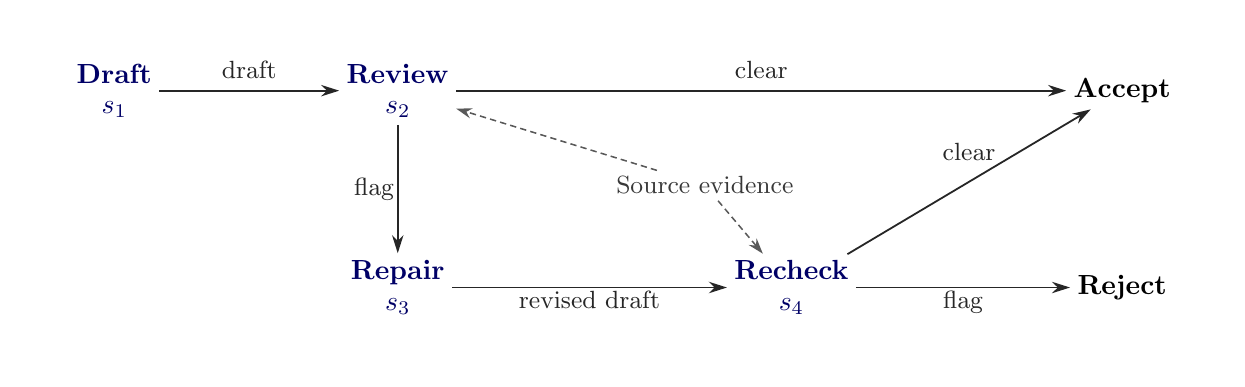
\begin{tikzpicture}[
  x=1mm,y=1mm,
  every node/.style={align=center, inner sep=2pt, outer sep=0pt},
  call/.style={text=blue!40!black, font=\normalsize},
  outcome/.style={text=black, font=\normalsize\bfseries},
  evidence/.style={text=black!78, font=\small},
  edge text/.style={text=black!85, font=\small, inner sep=1.4pt},
  execution/.style={
    draw=black!85, line width=.65pt,
    -{Stealth[length=2.3mm,width=1.45mm]}, shorten >=.7pt, shorten <=.7pt},
  source access/.style={
    draw=black!65, dash pattern=on 2.3pt off 1.5pt, line width=.55pt,
    -{Stealth[length=2mm,width=1.3mm]}, shorten >=.7pt, shorten <=.7pt}
]
  \path[use as bounding box] (-2,-34) rectangle (149,8);
  \node[call] (draft) at (9,0) {\textbf{Draft}\\[-.25ex]$s_1$};
  \node[call] (review) at (45,0) {\textbf{Review}\\[-.25ex]$s_2$};
  \node[call] (repair) at (45,-25) {\textbf{Repair}\\[-.25ex]$s_3$};
  \node[call] (recheck) at (95,-25) {\textbf{Recheck}\\[-.25ex]$s_4$};
  \node[outcome] (accept) at (137,0) {Accept};
  \node[outcome] (reject) at (137,-25) {Reject};
  \node[evidence] (source) at (84,-12) {Source evidence};

  \graph[use existing nodes, edges={execution}] {
    draft ->[edge node={node[edge text,above,yshift=1mm]{draft}}] review;
    review ->[edge node={node[edge text,above,yshift=1mm]{clear}}] accept;
    review ->[edge node={node[edge text,left]{flag}}] repair;
    repair ->[edge node={node[edge text,below]{revised draft}}] recheck;
    recheck ->[edge node={node[edge text,above,yshift=2.2mm]{clear}}] accept;
    recheck ->[edge node={node[edge text,below]{flag}}] reject;
  };
  \graph[use existing nodes, edges={source access}] {
    source -> review;
    source -> recheck;
  };
\end{tikzpicture}

\caption{Each call uses the settings $s_v$ in~\eqref{eq:settings}.
Dashed arrows give the reviewer and rechecker direct access to the source evidence.
A clear verdict accepts the draft under review.
The first flag sends the draft with feedback to repair.
The workflow rejects a draft flagged on recheck.}

\label{fig:graph}
\end{figure}

This conditional domain allows a parameter to become available only after its parent setting has been chosen.
Resolve defaults when freezing a configuration so that its identity determines the provider request.
Published suitability advice can guide the candidate proposals or supply predictive features.
Predicting its outcomes requires observations of the target task distribution.
A graph and its request settings determine a candidate to evaluate, while the evaluation supplies its outcome coefficients.

The topology can vary before any model is chosen.
Figure~\ref{fig:topologies} compares six ways to organise the calls and decisions.

\begin{figure}[htbp]
\centering
% Required packages: tikz
% Required TikZ libraries: arrows.meta
% Target width: 160 mm maximum
% Minimum text size: 8 pt
% Colour/greyscale intent: colour and greyscale
% Edge shafts: 0.7 pt
% Bold type redundantly identifies model calls.
% Positions mark connectivity. Distances do not represent time.
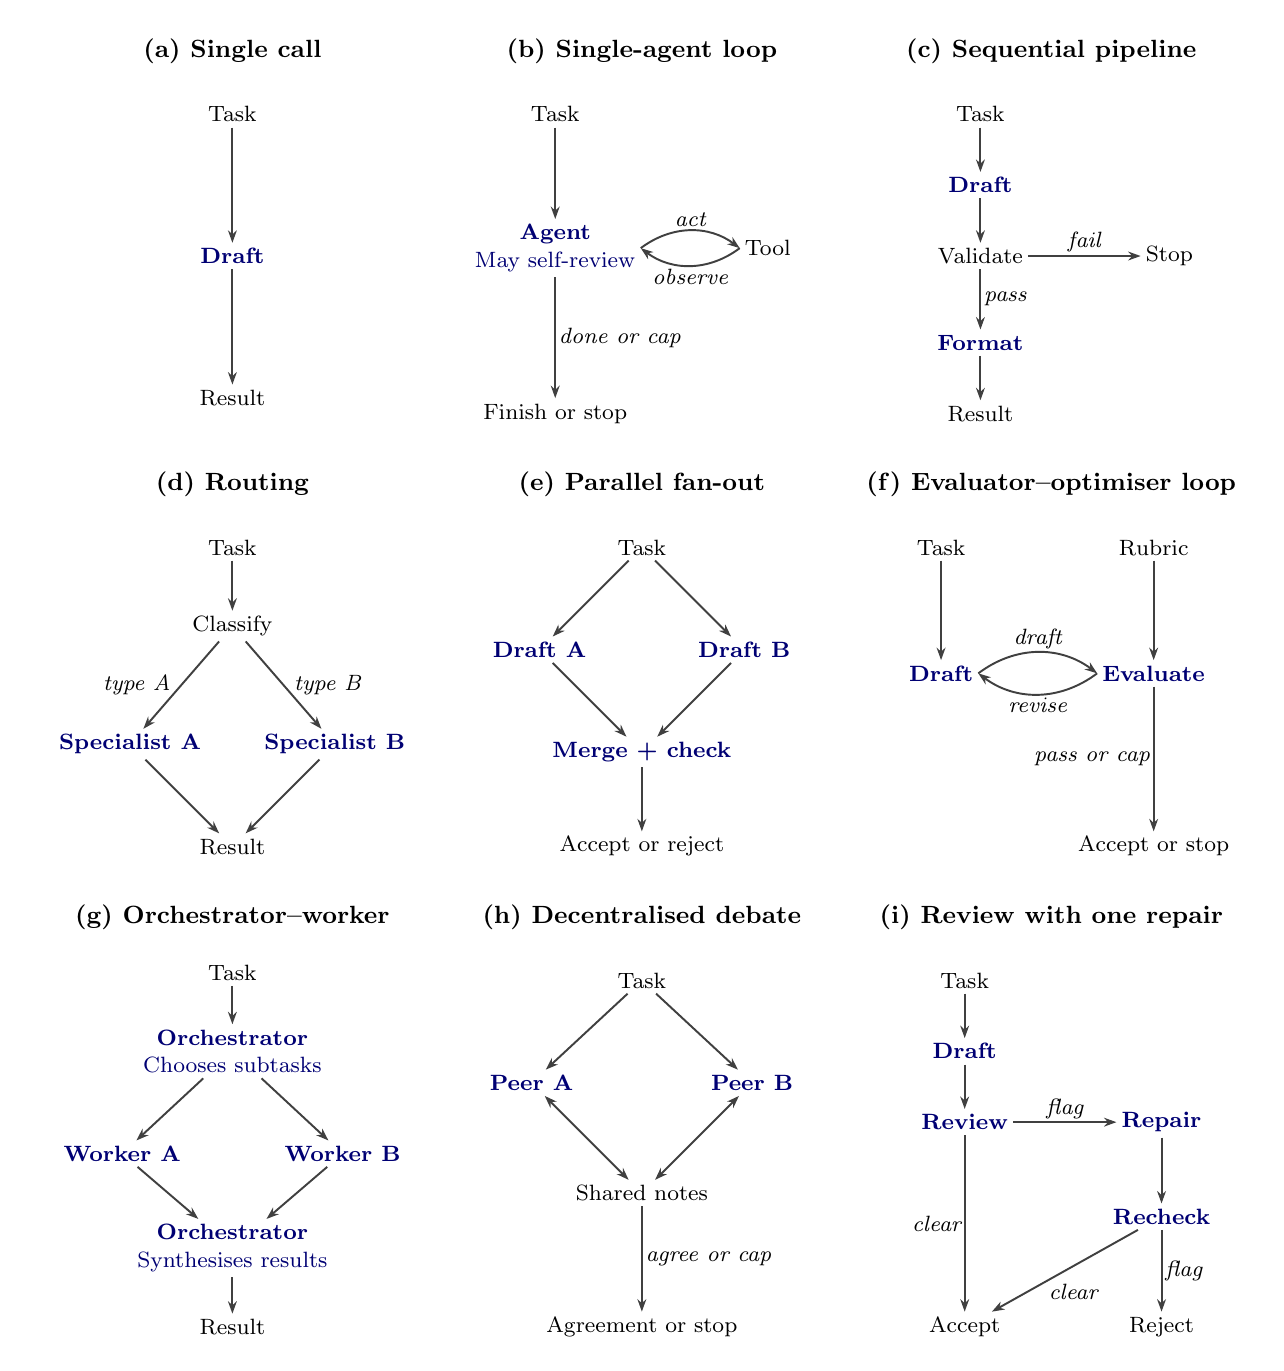
\begin{tikzpicture}[
  x=1mm,y=1mm,
  title/.style={font=\fontsize{9.5}{11}\selectfont\bfseries,inner sep=0pt},
  vertex/.style={font=\fontsize{8.5}{10}\selectfont,inner xsep=1.7pt,inner ysep=1.8pt,align=center},
  llm/.style={vertex,font=\fontsize{8.5}{10}\selectfont\bfseries,text=blue!45!black},
  condition/.style={font=\fontsize{8}{9}\selectfont\itshape,inner sep=1pt},
  flow/.style={->,draw=black!75,line width=.7pt,>={Stealth[length=4.5pt,width=3.2pt]}},
  exchange/.style={flow,<->},
]
\path[use as bounding box] (0,-164) rectangle (156,3);

\begin{scope}[xshift=26mm]
  \node[title] at (0,0) {(a) Single call};
  \node[vertex] (atask) at (0,-8) {Task};
  \node[llm] (adraft) at (0,-26) {Draft};
  \node[vertex] (aresult) at (0,-44) {Result};
  \draw[flow] (atask) -- (adraft);
  \draw[flow] (adraft) -- (aresult);
\end{scope}

\begin{scope}[xshift=78mm]
  \node[title] at (0,0) {(b) Single-agent loop};
  \node[vertex] (btask) at (-11,-8) {Task};
  \node[llm] (bagent) at (-11,-25) {Agent\\\textnormal{May self-review}};
  \node[vertex] (btool) at (16,-25) {Tool};
  \node[vertex] (bfinish) at (-11,-46) {Finish or stop};
  \draw[flow] (btask) -- (bagent);
  \draw[flow] (bagent.east) to[bend left=37] node[condition,above] {act} (btool.west);
  \draw[flow] (btool.west) to[bend left=37] node[condition,below] {observe} (bagent.east);
  \draw[flow] (bagent) -- node[condition,right] {done or cap} (bfinish);
\end{scope}

\begin{scope}[xshift=130mm]
  \node[title] at (0,0) {(c) Sequential pipeline};
  \node[vertex] (ctask) at (-9,-8) {Task};
  \node[llm] (cdraft) at (-9,-17) {Draft};
  \node[vertex] (cvalidate) at (-9,-26) {Validate};
  \node[vertex] (cstop) at (15,-26) {Stop};
  \node[llm] (cformat) at (-9,-37) {Format};
  \node[vertex] (cresult) at (-9,-46) {Result};
  \draw[flow] (ctask) -- (cdraft);
  \draw[flow] (cdraft) -- (cvalidate);
  \draw[flow] (cvalidate) -- node[condition,above] {fail} (cstop);
  \draw[flow] (cvalidate) -- node[condition,right] {pass} (cformat);
  \draw[flow] (cformat) -- (cresult);
\end{scope}

\begin{scope}[xshift=26mm,yshift=-55mm]
  \node[title] at (0,0) {(d) Routing};
  \node[vertex] (dtask) at (0,-8) {Task};
  \node[vertex] (droute) at (0,-18) {Classify};
  \node[llm] (dspeca) at (-13,-33) {Specialist A};
  \node[llm] (dspecb) at (13,-33) {Specialist B};
  \node[vertex] (dresult) at (0,-46) {Result};
  \draw[flow] (dtask) -- (droute);
  \draw[flow] (droute) -- node[condition,left,xshift=-2.5pt] {type A} (dspeca);
  \draw[flow] (droute) -- node[condition,right,xshift=2.5pt] {type B} (dspecb);
  \draw[flow] (dspeca) -- (dresult);
  \draw[flow] (dspecb) -- (dresult);
\end{scope}

\begin{scope}[xshift=78mm,yshift=-55mm]
  \node[title] at (0,0) {(e) Parallel fan-out};
  \node[vertex] (etask) at (0,-8) {Task};
  \node[llm] (edrafta) at (-13,-21) {Draft A};
  \node[llm] (edraftb) at (13,-21) {Draft B};
  \node[llm] (emerge) at (0,-34) {Merge + check};
  \node[vertex] (eresult) at (0,-46) {Accept or reject};
  \draw[flow] (etask) -- (edrafta);
  \draw[flow] (etask) -- (edraftb);
  \draw[flow] (edrafta) -- (emerge);
  \draw[flow] (edraftb) -- (emerge);
  \draw[flow] (emerge) -- (eresult);
\end{scope}

\begin{scope}[xshift=130mm,yshift=-55mm]
  \node[title] at (0,0) {(f) Evaluator--optimiser loop};
  \node[vertex] (ftask) at (-14,-8) {Task};
  \node[vertex] (frubric) at (13,-8) {Rubric};
  \node[llm] (fdraft) at (-14,-24) {Draft};
  \node[llm] (fevaluate) at (13,-24) {Evaluate};
  \node[vertex] (ffinish) at (13,-46) {Accept or stop};
  \draw[flow] (ftask) -- (fdraft);
  \draw[flow] (frubric) -- (fevaluate);
  \draw[flow] (fdraft.east) to[bend left=37] node[condition,above] {draft} (fevaluate.west);
  \draw[flow] (fevaluate.west) to[bend left=37] node[condition,below] {revise} (fdraft.east);
  \draw[flow] (fevaluate) -- node[condition,left] {pass or cap} (ffinish);
\end{scope}

\begin{scope}[xshift=26mm,yshift=-110mm]
  \node[title] at (0,0) {(g) Orchestrator--worker};
  \node[vertex] (gtask) at (0,-7) {Task};
  \node[llm] (gdispatch) at (0,-17) {Orchestrator\\\textnormal{Chooses subtasks}};
  \node[llm] (gworkera) at (-14,-30) {Worker A};
  \node[llm] (gworkerb) at (14,-30) {Worker B};
  \node[llm] (gcollect) at (0,-42) {Orchestrator\\\textnormal{Synthesises results}};
  \node[vertex] (gresult) at (0,-52) {Result};
  \draw[flow] (gtask) -- (gdispatch);
  \draw[flow] (gdispatch) -- (gworkera);
  \draw[flow] (gdispatch) -- (gworkerb);
  \draw[flow] (gworkera) -- (gcollect);
  \draw[flow] (gworkerb) -- (gcollect);
  \draw[flow] (gcollect) -- (gresult);
\end{scope}

\begin{scope}[xshift=78mm,yshift=-110mm]
  \node[title] at (0,0) {(h) Decentralised debate};
  \node[vertex] (htask) at (0,-8) {Task};
  \node[llm] (hpeera) at (-14,-21) {Peer A};
  \node[llm] (hpeerb) at (14,-21) {Peer B};
  \node[vertex] (hstate) at (0,-35) {Shared notes};
  \node[vertex] (hfinish) at (0,-52) {Agreement or stop};
  \draw[flow] (htask) -- (hpeera);
  \draw[flow] (htask) -- (hpeerb);
  \draw[exchange] (hpeera) -- (hstate);
  \draw[exchange] (hpeerb) -- (hstate);
  \draw[flow] (hstate) -- node[condition,right] {agree or cap} (hfinish);
\end{scope}

\begin{scope}[xshift=130mm,yshift=-110mm]
  \node[title] at (0,0) {(i) Review with one repair};
  \node[vertex] (itask) at (-11,-8) {Task};
  \node[llm] (idraft) at (-11,-17) {Draft};
  \node[llm] (ireview) at (-11,-26) {Review};
  \node[llm] (irepair) at (14,-26) {Repair};
  \node[llm] (irecheck) at (14,-38) {Recheck};
  \node[vertex] (iaccept) at (-11,-52) {Accept};
  \node[vertex] (ireject) at (14,-52) {Reject};
  \draw[flow] (itask) -- (idraft);
  \draw[flow] (idraft) -- (ireview);
  \draw[flow] (ireview) -- node[condition,left] {clear} (iaccept);
  \draw[flow] (ireview) -- node[condition,above] {flag} (irepair);
  \draw[flow] (irepair) -- (irecheck);
  \draw[flow] (irecheck) -- node[condition,below,xshift=3pt,yshift=-3.5pt] {clear} (iaccept);
  \draw[flow] (irecheck) -- node[condition,right] {flag} (ireject);
\end{scope}
\end{tikzpicture}

\caption{Bold labels identify model calls. A condition beside an arrow identifies
when that path is taken. Parallel calls can run together. In (g), the supervisor
has selected both workers. In (h), intake hands over when specialist review is
needed. In (i), crossing arrows carry peer messages and dashed arrows carry local
state into the next round. A deterministic check accepts matching results and
rejects disagreement. The simulation uses the single-call baseline in (a) and
the multi-call workflows in (c) and (d). The other panels illustrate additional
arrangements.}

\label{fig:topologies}
\end{figure}

Let $g\in\{1,\ldots,n_g\}$ identify a task group observed before routing and let $k\in\{1,\ldots,K\}$ identify an operating scenario.
The known task-group proportions satisfy $\mu_{gk}\ge0$ and $\sum_g\mu_{gk}=1$.
A scenario specifies a task distribution together with operating conditions relevant to the workflow outcomes.
The router observes $g$ and uses a common selection rule across scenarios.

If further information is available for routing, incorporate it into the group definition or the complete workflow.

Let $A\in\{0,1\}$ indicate acceptance and let $Y\in\{0,1\}$ indicate acceptance of an output containing a material defect.
A rejected execution has $Y=0$, so $Y\le A$.
Material-defect criteria are fixed before evaluation.
Interpreting the labels as defects requires reliable independent assessment or a validated model of labelling error.
For total cost $C\ge0$ and elapsed time $T\ge0$, define lateness by $L=\mathbf1\{T>d\}$ at deadline $d>0$.
Both cost and lateness count every attempted task.
A late output contributes to acceptance when the acceptance rule allows it.
If useful completion requires an on-time output, encode that condition in $A$ before collecting observations.

For configuration $\theta_j$, define
\begin{equation}
 \begin{aligned}
 a_{gjk}&=\mathbb E[A\mid g,\theta_j,k],&
 b_{gjk}&=\mathbb E[Y\mid g,\theta_j,k],\\
 c_{gjk}&=\mathbb E[C\mid g,\theta_j,k],&
 \ell_{gjk}&=\mathbb E[L\mid g,\theta_j,k].
 \end{aligned}
 \label{eq:outcomes}
\end{equation}
Thus $0\le b_{gjk}\le a_{gjk}\le1$, $0\le\ell_{gjk}\le1$ and $c_{gjk}<\infty$.
The cost boundary includes task classification and orchestration.
A cell with $\mu_{gk}=0$ contributes zero, so any coefficients satisfying these ranges may be assigned to it.

\begin{assumption}[Deployment validity]\label{ass:deployment}
Every configuration terminates almost surely and has finite expected cost.
Conditional on $g$, the router selects a configuration using fresh randomness independent of the remaining task characteristics and execution randomness.
For every allowed routing rule, the conditional coefficients in~\eqref{eq:outcomes} remain valid under the operating conditions represented by each scenario.
\end{assumption}

The last condition makes the measured workflow outcomes applicable to deployment.
It requires evidence when configurations share a capacity-limited provider or queue.
A fixed scenario label supplies a modelling index, while measurements or a justified system model establish that its coefficients remain valid as the routing mix changes.

\section{Constrained selection among complete graphs}
\label{sec:selection}

Let $\Theta_J=\{\theta_1,\ldots,\theta_J\}$ be a finite candidate set.
The weight $w_{gj}$ is the probability of selecting configuration $j$ for group $g$.
Write
\begin{equation}
 \mathcal W_J=
 \left\{w\in\mathbb R^{n_g\times J}:\ w_{gj}\ge0,
              \ \sum_jw_{gj}=1\ \text{for every }g\right\}.
 \label{eq:simplex}
\end{equation}
For any cell quantity $v\in\{a,b,c,\ell\}$, its scenario aggregate is
\begin{equation}
 v_k(w)=\sum_{g=1}^{n_g}\sum_{j=1}^{J}\mu_{gk}w_{gj}v_{gjk}.
 \label{eq:mixture}
\end{equation}
When $a_k(w)>0$, the defect fraction among accepted outputs is $q_k(w)=b_k(w)/a_k(w)$.

\begin{lemma}[Mixture outcomes]\label{lem:mixture}
Under Assumption~\ref{ass:deployment}, equation~\eqref{eq:mixture} gives the outcome moments of the deployed rule.
If $a_k(w)>0$, then
\begin{equation}
 q_k(w)=
 \sum_{\{(g,j):\,a_{gjk}>0\}}
 \frac{\mu_{gk}w_{gj}a_{gjk}}{a_k(w)}
 \frac{b_{gjk}}{a_{gjk}}.
 \label{eq:accepted-mixture}
\end{equation}
\end{lemma}
\begin{proof}
The probability of entering cell $(g,j)$ in scenario $k$ is $\mu_{gk}w_{gj}$.
Conditioning on that cell gives~\eqref{eq:mixture} by total expectation.
If $a_{gjk}=0$, the inequality $b_{gjk}\le a_{gjk}$ gives $b_{gjk}=0$.
Removing these zero contributions and dividing the sum for $b_k(w)$ by $a_k(w)$ proves~\eqref{eq:accepted-mixture}.
Its coefficients sum to one.
\end{proof}

The weights in~\eqref{eq:accepted-mixture} describe the accepted population.
A configuration that accepts more often contributes more accepted outputs for the same share of attempts.
Measuring the complete workflow preserves dependence between its stages before these outcomes are mixed.

Fix a defect tolerance $\varepsilon\in[0,1]$, a completion floor $\gamma\in(0,1]$ and a lateness ceiling $\delta\in[0,1]$.
The deployment programme is
\begin{equation}
 \begin{aligned}
 \underset{w,z}{\operatorname{minimise}}\quad &z\\
 \text{subject to}\quad
 &c_k(w)\le z &&(k=1,\ldots,K),\\
 &b_k(w)-\varepsilon a_k(w)\le0 &&(k=1,\ldots,K),\\
 &a_k(w)\ge\gamma &&(k=1,\ldots,K),\\
 &\ell_k(w)\le\delta &&(k=1,\ldots,K),\\
 &w\in\mathcal W_J.
 \end{aligned}
 \label{eq:master}
\end{equation}
Each weight refers to a complete graph with its model settings, so this selection determines the deployed proportions of those designs.
The epigraph variable $z\in\mathbb R$ bounds expected cost in every scenario.

\begin{theorem}[Finite-configuration optimum]\label{thm:master}
Under Assumption~\ref{ass:deployment}, programme~\eqref{eq:master} is a linear programme with $n_gJ+1$ variables.
It is equivalent to minimising $\max_kc_k(w)$ subject to the population requirements $q_k(w)\le\varepsilon$, $a_k(w)\ge\gamma$ and $\ell_k(w)\le\delta$ for every scenario.
Whenever its feasible set is nonempty, it attains a finite global minimum over $\Theta_J$.
\end{theorem}
\begin{proof}
The completion constraint gives $a_k(w)\ge\gamma>0$.
Consequently
\[
 \frac{b_k(w)}{a_k(w)}\le\varepsilon
 \quad\Longleftrightarrow\quad
 b_k(w)-\varepsilon a_k(w)\le0.
\]
All aggregates are linear in $w$, and $\varepsilon$ is fixed.
For any feasible $w$, the smallest allowed value of $z$ is $\max_kc_k(w)$.
This establishes equivalence and linearity.
The feasible weights form a closed subset of the compact set $\mathcal W_J$.
The maximum of finitely many finite linear cost functions is continuous, so it attains its minimum on that subset whenever the subset is nonempty.
\end{proof}

The theorem supplies an optimum for the candidate set presented to the solver.
Finding a better graph enlarges that set and can change the optimum.
If deployment requires one configuration per group, impose binary weights with the same row sums.
That requirement gives a mixed-integer selection problem and may change feasibility.

\paragraph{Requirements for each task group.}
Write $v_{gk}(w)=\sum_j w_{gj}v_{gjk}$ for a conditional outcome.
When each task group requires the same service, impose
\[
 a_{gk}(w)\ge\gamma,\qquad
 b_{gk}(w)-\varepsilon a_{gk}(w)\le0,\qquad
 \ell_{gk}(w)\le\delta
 \quad (\mu_{gk}>0).
\]
The objective still uses scenario-wide cost $c_k(w)$.
Multiplying the group inequalities by $\mu_{gk}$ and summing recovers the original scenario-wide inequalities.
Thus the group requirements can raise cost or make the programme infeasible.
The same simultaneous cell bounds also protect the group programme, because its row weights are nonnegative.

\begin{proposition}[Dominance screening and sparse routing]\label{prop:reduction}
For a fixed group and defect tolerance, consider the column with entries
$(c_{gjk},b_{gjk}-\varepsilon a_{gjk},-a_{gjk},\ell_{gjk})$ across all scenarios with $\mu_{gk}>0$.
A column can be removed if a retained column for that group is no greater in any entry.
For the scenario-wide master programme, an optimal vertex with $p$ positive weights and $m$ binding scenario inequalities satisfies
$p\le n_g+m-1\le n_g+4K-1$.
\end{proposition}
\begin{proof}
Transferring the removed column's weight to its replacement preserves the group sum and weakly decreases every left-hand side at fixed $z$.
Apply this argument separately to each removed column, keeping one representative of any tied columns.
The feasible epigraph is a pointed polyhedron because its weights are bounded and its only possible vertical recession direction increases $z$.
A finite attained minimum therefore has an optimal vertex.
After fixing the zero weights, a vertex has $p+1$ free coordinates including $z$.
Its $n_g$ group equalities and $m$ binding inequalities must span those coordinates.
Otherwise a small perturbation in either direction along a common null vector preserves feasibility, contradicting extremality.
\end{proof}

The dominance test also applies to the group rows above and to fixed calibration coefficients.
Recompute it whenever the coefficients or tolerance change.
An ordering based on cost, joint defects, negative acceptance and lateness is sufficient for all nonnegative tolerances.
The fixed-tolerance test can remove additional columns.
A direct pairwise implementation takes $O(n_gKJ^2)$ comparisons of scalar coefficients.
It reduces the master problem after coefficients are available.
Before evaluation it needs structural evidence, such as an identical execution law with a higher tariff.
The sparse optimum can aid deployment even when screening removes few configurations.
If the policy needs a particular number of active configurations or prohibits immediate rejection, put that requirement in the optimisation.

\begin{proposition}[Fixed-budget search]\label{prop:budget}
For $B\ge0$, let $\mathcal W_B$ contain the weights satisfying $c_k(w)\le B$, $a_k(w)\ge\gamma$ and $\ell_k(w)\le\delta$ for every scenario.
If $\mathcal W_B$ is nonempty, the value
\[
 q_B^*=\min_{w\in\mathcal W_B}\max_k\frac{b_k(w)}{a_k(w)}
\]
is attained in $[0,1]$.
For fixed $\varepsilon\in[0,1]$, the inequality $q_B^*\le\varepsilon$ holds exactly when~\eqref{eq:master} is feasible with $z\le B$.
Feasibility is monotone in $\varepsilon$.
\end{proposition}
\begin{proof}
The set $\mathcal W_B$ is compact and each denominator is at least $\gamma$.
The objective is therefore continuous and attains its minimum.
The linear risk conversion used in Theorem~\ref{thm:master} proves the feasibility equivalence.
For $\varepsilon'\ge\varepsilon$, nonnegative acceptance gives
$b_k(w)-\varepsilon'a_k(w)\le b_k(w)-\varepsilon a_k(w)$.
Thus increasing the tolerance preserves feasibility.
\end{proof}

With exact feasibility decisions, checking the endpoints $0$ and $1$ establishes an initial bracket or identifies a zero optimum.
Bisection then gives a feasible upper endpoint within a bracket of width $\eta$ after at most $\lceil\log_2(1/\eta)\rceil$ midpoint checks, for $0<\eta<1$.
A conservative programme using confidence bounds certifies feasibility through those bounds.
Its failure leaves population feasibility open.

For one scenario there is also an exact one-LP reduction \cite{boyd,charnesCooper}.
Write the fixed-budget feasible set as $Dw\le h$, $Ew=\mathbf 1$, $w\ge0$.
With $t=1/a(w)$ and $x=tw$, minimise $b(x)$ subject to
$Dx\le ht$, $Ex=t\mathbf 1$, $a(x)=1$, $x\ge0$ and $t\ge0$.
The equalities force $t>0$, so $w=x/t$ recovers a feasible rule with the same objective.
This is the Charnes--Cooper transformation.
One scaling also works across scenarios when their denominators are positive fixed multiples of a common linear function.
For general scenario-specific denominators the paper uses the LP feasibility search above.
In the adverse scenario of Appendix~\ref{app:exact} alone, a budget of $13/10$
gives minimum risk $123/1300$ at the appendix's completion and lateness limits.
The accompanying check recovers the same value with one transformed LP,
bisection and an exact rational lower bound.

\section{Calibration after graph search}
\label{sec:calibration}

Development data can determine the candidate set and guide its search.
For the construction below, freeze that set and the task classifier before collecting calibration observations.
Condition on the completed development stage when constructing the bounds.
The task proportions are known, or their uncertainty is included in a justified extension of the scenario set.

Suppose the calibration procedure supplies simultaneous bounds with probability at least $1-\alpha$, where $0<\alpha<1$,
\begin{equation}
 \mathcal E=\left\{
 a^-_{gjk}\le a_{gjk},\quad
 b_{gjk}\le b^+_{gjk},\quad
 c_{gjk}\le c^+_{gjk},\quad
 \ell_{gjk}\le\ell^+_{gjk}
 \text{ for all relevant cells}\right\}.
 \label{eq:coverage}
\end{equation}
Aggregate these endpoints using~\eqref{eq:mixture}.
The conservative programme replaces the cost and lateness coefficients by their upper bounds.
It also requires $a_k^-(w)\ge\gamma$ and $b_k^+(w)\le\varepsilon a_k^-(w)$.

\begin{theorem}[Validity after data-dependent selection]\label{thm:calibration}
Assume~\eqref{eq:coverage} and Assumption~\ref{ass:deployment}.
On $\mathcal E$, every routing rule feasible for the conservative programme satisfies the corresponding true population requirements.
The assertion holds simultaneously for every subsequent choice of weights and every nonnegative defect tolerance.
A procedure that returns only a feasible rule has probability at most $\alpha$ of returning a rule that violates a population requirement.
\end{theorem}
\begin{proof}
The coefficients $\mu_{gk}w_{gj}$ are nonnegative, so their weighted sums preserve each inequality in~\eqref{eq:coverage}.
In particular,
\[
 b_k(w)-\varepsilon a_k(w)
 \le b_k^+(w)-\varepsilon a_k^-(w)\le0,
 \qquad
 a_k(w)\ge a_k^-(w)\ge\gamma>0.
\]
Division by $a_k(w)$ proves the risk requirement.
The cost and lateness conclusions follow by the same weighted sums.
These implications hold for every feasible rule on the same event $\mathcal E$, including a rule selected using the calibration data.
Returning a violating rule therefore requires $\mathcal E^c$, which has probability at most $\alpha$.
If the development stage is random, integrate the same conditional bound over that stage.
\end{proof}

This is the uniform-bound selection argument discussed in Learn then Test~\cite{ltt}.
The probability statement concerns the full procedure over repeated calibration samples.
Conditioning on the event that a rule was returned can change its error probability.
The conservative cost optimum supplies a population cost upper bound, while its gap from the minimum true cost remains unresolved.

A simple construction uses $N$ nonempty cells.
In cell $i$, take $n_i\ge1$ independent draws from that cell's population with an actual cost range $0\le C\le C_{\max,i}$.
Choose the sample sizes and sampling plan independently of calibration outcomes.
Let $\bar a_i$, $\bar b_i$, $\bar c_i$ and $\bar\ell_i$ be empirical means of the observed quantities.
Set
\begin{equation}
 \begin{gathered}
 r_i=\sqrt{\frac{\log(4N/\alpha)}{2n_i}},\\
 a_i^- =\max\{0,\bar a_i-r_i\},\qquad
 b_i^+ =\min\{1,\bar b_i+r_i\},\\
 \ell_i^+=\min\{1,\bar\ell_i+r_i\},\qquad
 c_i^+=\min\{C_{\max,i},\bar c_i+C_{\max,i}r_i\}.
 \end{gathered}
 \label{eq:hoeffding}
\end{equation}
Hoeffding's inequality bounds each one-sided failure probability by $\alpha/(4N)$~\cite{hoeffding}.
A union bound over the $4N$ endpoints proves~\eqref{eq:coverage}.
The union bound permits dependence between cells, while the within-cell sampling assumptions still apply.
Known deterministic outcomes can use exact coefficients.
Outcome-dependent stopping requires a valid sequential construction.
A finite cost bound must follow from the actual execution and billing rules.

\paragraph{Paired calibration at a fixed defect limit.}
Fix $\varepsilon$ before calibration and observe the signed score
$Z_\varepsilon=Y-\varepsilon A$ on each attempted task.
Its three possible values are $0$, $-\varepsilon$ and $1-\varepsilon$.
An upper bound $u_i(\varepsilon)$ on its cell mean can directly supply the risk coefficient.
On simultaneous coverage, the true risk row is bounded above by the corresponding weighted sum of the $u_i(\varepsilon)$.
The acceptance lower bound still supplies the positive denominator.
Use $\alpha/(4N)$ for each of the four bounds per cell, with one bound each for completion, signed risk, cost and lateness.

Since $Z_\varepsilon$ has range width one, the one-sided Hoeffding construction gives
$u_i(\varepsilon)=\min\{1-\varepsilon,\bar b_i-\varepsilon\bar a_i+r_i\}$.
This bound is at most $b_i^+-\varepsilon a_i^-$ for every sample.
When $\bar b_i+r_i\le1$, this follows from $a_i^-\le\bar a_i$.
When $\bar b_i+r_i>1$, the separate coefficient is at least $1-\varepsilon$.
At fixed tolerance and otherwise identical bounds, the paired Hoeffding LP therefore has a weakly lower optimum whenever the separate LP is feasible.
Known deterministic outcomes use their exact scores.

A variance-sensitive alternative uses Maurer and Pontil's empirical Bernstein bound~\cite[Theorem~4]{maurerPontil} for $Z_\varepsilon+\varepsilon\in[0,1]$.
For $n_i\ge2$ and $\xi=\alpha/(4N)$, use
\[
 u_i(\varepsilon)=\min\left\{1-\varepsilon,\ \bar Z_i+
 \sqrt{\frac{2s_i^2\log(2/\xi)}{n_i}}+
 \frac{7\log(2/\xi)}{3(n_i-1)}\right\},
\]
where $s_i^2$ is the ordinary sample variance of the paired scores.
Either bound gives the same simultaneous risk guarantee for a prespecified method and tolerance.
Empirical Bernstein can be wider than Hoeffding.
Choosing a bound after seeing the data requires simultaneous protection for that choice.
For a tolerance selected after calibration, retain the separate endpoints or protect the paired bounds jointly over a prespecified finite grid.

\section{Dual-guided search over configurations}
\label{sec:pricing}

An enumerated candidate space can exceed the evaluation budget even when each deployment LP is small.
Column generation gives a way to direct the next evaluation using the current decision~\cite{dantzigwolfe}.
Let $\Theta_0$ be a restricted subset of a larger finite admissible set $\Theta$.
Assume the restricted programme is feasible and use fixed coefficients throughout the comparison.
For its optimal dual solution, let $\lambda_k$, $\beta_k$, $\kappa_k$ and $\nu_k$ be the nonnegative multipliers of the cost, risk, completion and lateness inequalities.
The free multiplier $\zeta_g$ corresponds to $1-\sum_jw_{gj}=0$.
Define the reduced cost of configuration $\theta$ for task group $g$ by
\begin{equation}
 R_g(\theta)=
 \sum_k\mu_{gk}
 \left\{
 \lambda_kc_{g\theta k}
 +\beta_k\bigl(b_{g\theta k}-\varepsilon a_{g\theta k}\bigr)
 -\kappa_ka_{g\theta k}
 +\nu_k\ell_{g\theta k}
 \right\}-\zeta_g.
 \label{eq:reduced-cost}
\end{equation}
The multipliers express the value of a candidate's outcomes under the currently binding service requirements.

\begin{proposition}[Pricing certificate]\label{prop:pricing}
The optimal restricted dual solution satisfies $\sum_k\lambda_k=1$.
If $R_g(\theta)\ge0$ for every $g$ and every $\theta\in\Theta$, the restricted primal solution is optimal over $\Theta$.
More generally, if known values $\sigma_g\ge0$ satisfy $R_g(\theta)\ge-\sigma_g$ throughout $\Theta$, the restricted cost exceeds the full-space optimum by at most $\sum_g\sigma_g$.
\end{proposition}
\begin{proof}
The coefficient of the free epigraph variable $z$ in the Lagrangian is $1-\sum_k\lambda_k$.
Dual feasibility therefore requires its vanishing.
The coefficient of a nonnegative routing variable is~\eqref{eq:reduced-cost}.
If every such coefficient is nonnegative throughout $\Theta$, the restricted dual solution is also feasible for the full programme.
Its objective equals the restricted primal objective by finite-dimensional linear-programming duality.
The restricted primal solution is feasible for the full programme, so weak duality gives equality of the two optima.
For the approximate statement, replace each $\zeta_g$ by $\zeta_g-\sigma_g$.
Every reduced cost becomes nonnegative, giving a full-programme dual lower bound smaller by $\sum_g\sigma_g$.
\end{proof}

A negative reduced cost identifies a graph to consider adding.
Degeneracy can make its immediate objective improvement zero.
A surrogate can rank unevaluated graphs by predicted reduced cost and uncertainty, after which complete executions supply their coefficients.
Such a search gives an optimum over the candidates retained for the LP.
The full-space certificate in Proposition~\ref{prop:pricing} requires a bound covering every admissible candidate.
For conservative coefficients, substitute $c^+$, $b^+$, $a^-$ and $\ell^+$ in~\eqref{eq:reduced-cost} and keep those endpoints fixed during the comparison.
Fresh calibration after the candidate set is frozen provides the statistical treatment used in Theorem~\ref{thm:calibration}.



\section{Published guidance and outcome prediction}
\label{sec:prediction}
A model registry supplies the domain of valid node configurations.
Store an exact model identifier together with its endpoint and the date of the capability source.
A supported reasoning setting activates the remaining compatible parameters.
A model whose endpoint has no adjustable reasoning control has a singleton reasoning domain and remains eligible.
Provider documentation supplies these domains, while its recommended uses can influence which candidates the search evaluates first \cite{openai_reasoning,anthropic_effort,gemini_thinking}.

A recommendation for difficult programming tasks supplies a proposal preference.
It leaves the defect probability on a particular release-note task to be estimated.
One implementation assigns a suitability score to a candidate and samples from a softmax of these scores, mixed with a distribution that gives every eligible candidate positive probability.
The exploration component allows observed outcomes to overturn the initial preference.
An experiment comparing search with and without the advice features can assess whether those features reduce evaluation cost.

For an observed input description $x$, let $\phi(x,\theta,k)$ encode the task and candidate graph in scenario $k$.
The representation needs to distinguish nodes by role and setting.
It also needs to preserve consequential source-access paths and repair conditions.
Fit a joint outcome predictor
\begin{equation}
(p_R,p_G,p_B)=\softmax f_\psi(\phi(x,\theta,k)),
\qquad \widehat a=p_G+p_B,\qquad \widehat b=p_B,
\label{eq:predictor}
\end{equation}
where $R$ denotes rejection, $G$ acceptance without a material defect, and $B$ acceptance with a material defect.
The three probabilities sum to one, giving $0\le\widehat b\le\widehat a\le1$.
Average task-level predictions over the relevant group distribution before using them as selection coefficients.
Features used for this prediction must be available before the candidate runs, or integrated out by another justified model.

A conditional-mean model supplies expected cost.
For a fixed deadline, a binary classifier can estimate lateness.
When the deadline itself varies, a completion-time distribution $F_T$ supplies $\ell(d)=1-F_T(d)$.
A timestamp beyond a hard timeout has a different interpretation from an observation whose eventual completion time is unknown.
The outcome definition and estimation procedure must preserve that distinction.

The predictive model is a component to assess on withheld tasks and graph configurations.
A regularised predictor with graph interactions and a tree-based surrogate provide accessible initial comparisons.
A graph neural predictor requires enough measured graph variation to learn and test its structural effects.
The simulation below evaluates the selection calculations using known synthetic coefficients and sampled calibration data.
Choosing a predictive model for unexecuted production graphs remains a subsequent empirical step.

\section{A finite simulation with published configurations}
\label{sec:simulation}
We use a finite synthetic experiment to check the computation, expose the
effect of calibration uncertainty and make every outcome assumption inspectable.
No LLM is called. Provider documentation supplies model identifiers, compatible
controls and token prices. We stipulate the quality, token usage and duration laws.
The pool contains three model identifiers, three graph families, three effort
settings and two output caps, plus immediate rejection, giving $J=55$ candidates.
Panels (a), (c) and (d) of Figure~\ref{fig:topologies} show the basic paths in these families.
Every node within a graph shares its model, effort and cap. This is a restricted
subspace of the proposed node-wise configuration domain.

\begin{table}[H]
\centering
\small
\begin{tabular}{lll}
\toprule
Model identifier & Efforts used & Input/output USD per million tokens\\
\midrule
\texttt{gpt-6.1-sol} & low, medium, high & 2.00 / 10.00\\
\texttt{claude-sonnet-5-5} & low, medium, high & 2.00 / 10.00\\
\texttt{gemini-4-hydrogen} & low, medium, high & 1.50 / 7.50\\
\bottomrule
\end{tabular}
\caption{Dated registry inputs verified on 13 November 2026. Selected per-call
generated-token caps are 4,096 and 8,192. Endpoint-specific parameter names and
compatibility restrictions are retained in the machine-readable registry.
The experiment uses short, uncached inputs at standard quoted rates
\cite{openaiSol2026,openaiDeploy2026,anthropicSonnet2026,googlePricing2026,googleHydrogen2026}.
The numerical quality and duration laws do not come from these sources.}
\label{tab:registry}
\end{table}

\paragraph{Whole-graph outcome mechanism.}
Let $g=0,1$ denote supplied routine and migration labels, and let $k=0,1$
denote unobserved nominal and adverse scenarios. Group proportions are
$(0.70,0.30)$ and $(0.40,0.60)$ respectively. Classification and orchestration
overheads are zero. Each attempt draws difficulty $D$, blind spot $B$ and
slow load $S$ according to
\[
\begin{aligned}
\Pr(D=1\mid g,k)&=0.15+0.40g+0.10k,\\
\Pr(B=1\mid D,k)&=0.01+0.02D+0.01k,\\
\Pr(S=1\mid k)&=0.06+0.08k.
\end{aligned}
\]
Load is independent of $(D,B)$. Every node shares these states.
Conditional error and checking draws follow the rules below.
Their residual Bernoulli randomness is independent conditional on the shared states and the defect status inherited by each operation.
This gives parallel and repeated calls common failure causes.

For effort $e\in\{\mathrm{low},\mathrm{medium},\mathrm{high}\}$, the draft
defect probability is $1$ if $B=1$, and otherwise
$(0.12+0.26D+0.06k)(1,0.62,0.35)_e$.
A check detects a defect with probability $0.08$ under a blind spot and
$(0.65,0.82,0.94)_e-0.08D$ otherwise. Its false-alarm probability is $0.03$.
The single graph accepts a completed draft. The serial graph reviews its
draft and, only when flagged, performs one repair followed by a final review.
Repair has defect probability one under a blind spot and $0.65$ times the
draft defect probability otherwise. A final flag rejects the result.
The parallel graph produces two simultaneous drafts and merges them.
Outside a blind spot, merge defect probabilities are
$(0.85,0.70,0.55)_e$ for two defective drafts,
$(0.25,0.14,0.07)_e+0.04D$ for one, and $0.01+0.01D$ for neither.
Under a blind spot the merge is defective. Merge checks its own result
within the same call and rejects on a flag.

The script specifies role-dependent input and generated-token counts.
The selected output cap limits the synthetic billable generated count,
including reasoning tokens once. Visible answer tokens form only part of this count.
A call whose desired generated count exceeds its cap is truncated and causes
rejection under the graph rules. This cap-to-rejection law is an assumption
of the simulator. For input count $I$, capped generated count $U$ and registry
prices $p_{\rm in},p_{\rm out}$, its charge and duration are
\[
C_v=10^{-6}(p_{\rm in}I+p_{\rm out}U),\qquad
T_v=(1+0.7S)(2+0.008I+0.012U)\ \mathrm{s}.
\]
Charges add over executed calls. Serial durations add, while parallel draft
duration is their maximum. Both drafts have the same duration conditional
on the shared state in this experiment. Rejection retains incurred cost
and duration. Immediate rejection has zero cost and duration. The terminal
distribution is finite, so all population coefficients are obtained by
enumeration, up to floating-point arithmetic. The full constants and all
terminal outcomes accompany the code.

\paragraph{Selection and calibration.}
The service requirements are $\gamma=0.80$, $\varepsilon=0.10$,
$\delta=0.15$ and $d=180\,\mathrm{s}$. Acceptance and lateness are separate
events. An accepted late output counts in both. The same routing weights
must satisfy both scenarios. Quality and duration laws are identical across
provider identities, and their usage laws are also identical. Therefore
selection of the cheaper registry entry follows from this assumption.
Provider quality comparisons require measured outcomes.

The exact full-pool optimum costs USD~0.0387983 per attempted task in its
worst scenario. There, acceptance is $0.80$, defects among accepted outputs
are $0.10$, and lateness is $0.15$. All three constraints bind.
The single-call pool is infeasible at these limits.
Figure~\ref{fig:simulation-frontier} varies only the defect limit.
Figure~\ref{fig:simulation-routing} shows the optimal routing weights.
The completion constraint is aggregate within each scenario. It permits
30.39\% immediate rejection in the migration group. In the adverse scenario,
migration completion is 67.99\% and its lateness is 16.14\%.
Routine tasks have 10.17\% defects among accepted outputs in that scenario.
Requiring the same three limits in each nonempty group and scenario gives
a population optimum of USD~0.0423768 per attempt, 9.22\% above the
scenario-wide baseline. The group constraints express a service policy.
They apply when the stated limits are intended for every group.

At fixed tolerance, dominance screening retains 10 columns per group from 55.
The reduced LP recovers the full optimum to within $10^{-10}$ USD.
The returned aggregate solution uses five positive weights, within the bound
of nine from Proposition~\ref{prop:reduction}.
The screening uses already enumerated coefficients. This experiment measures the
reduction in LP size. Evaluation savings would require a structural test before execution.

For the primary frozen-pool calibration, the 216 uncertain
group--candidate--scenario cells each receive 20,000 independent synthetic
trials, giving 4.32 million in total. A multinomial draw from each finite terminal
distribution supplies the sample counts. Immediate rejection is exactly
known. With family error $\alpha=0.05$, the one-sided Hoeffding radius is
$0.0156183$. The finite execution distribution provides the required cost
bound. The bound-based LP has a worst-scenario cost upper bound of
USD~0.0468272 per attempt. Exact evaluation of that selected rule gives
worst-scenario cost USD~0.0455392, accepted-defect risk $0.0824426$,
minimum acceptance $0.812269$ and maximum lateness $0.137539$.
All simultaneous bounds contain their population values in this seeded
realisation. This checks the calculated bounds for one sample, while the
coverage guarantee follows from Theorem~\ref{thm:calibration}.
On the same 20,000 trials per cell, the paired Hoeffding risk bound gives
a cost upper bound of USD~0.0459774 per attempt. Paired empirical Bernstein
gives USD~0.0433804, 7.36\% below the separate Hoeffding bound.
With per-group service constraints, the corresponding bounds are
USD~0.0521947, USD~0.0515283 and USD~0.0491695 for separate Hoeffding,
paired Hoeffding and paired empirical Bernstein respectively.
Each method has its own 95\% simultaneous guarantee given its assumptions.
On this sample all three sets of bounds contain the stipulated cell coefficients.
Figure~\ref{fig:simulation-calibration} retains the separate Hoeffding
comparison across sample sizes, with one independently seeded sample per size.

An exact reduced-cost search starts from the 18 single-call candidates,
rejection and a fixed serial/high/8,192 feasibility seed. Three additions
bring the restricted pool from 20 to 23 candidates. Its fourth solve matches
the full-pool objective within $10^{-10}$ USD. Every omitted candidate is
priced using already-known coefficients. This checks column generation over
the finite pool. The experiment leaves evaluation savings and the
predictive benefit of published advice to be tested.

\begin{figure}[tbp]
\centering
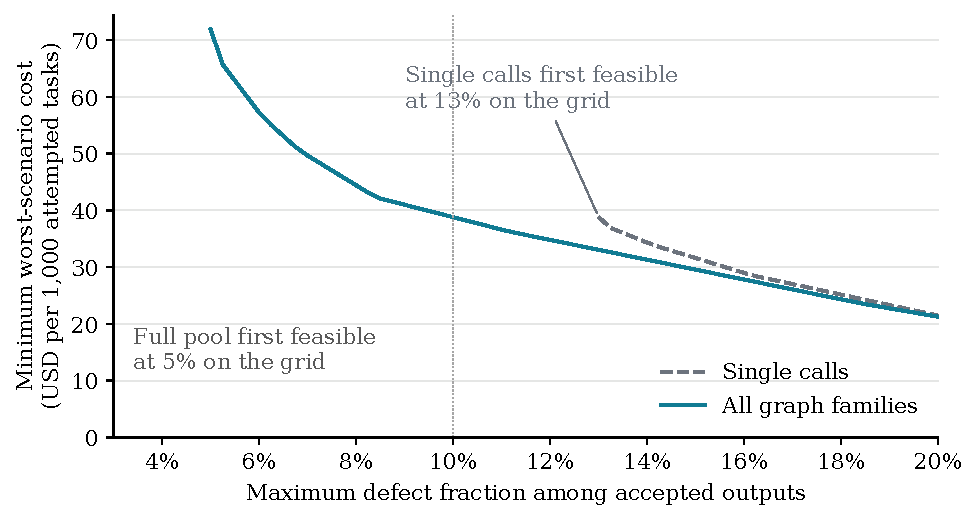
\includegraphics[width=\linewidth]{figures/cost-risk-frontier.pdf}
\caption{Minimum worst-scenario cost in the finite synthetic experiment.
Each point uses exact population coefficients, acceptance at least 80\%,
and at most 15\% of attempts exceeding 180\,s in both scenarios.
The solid curve uses all 55 candidates. The dashed curve uses 18 single-call
configurations and rejection. Costs include rejected attempts. Curves connect
thresholds spaced by 0.25 percentage points. Infeasible sampled thresholds
are omitted and labelled. The first feasible grid points are 5\% for the
full pool and 13\% for single calls. At 10\%, the full pool costs USD~38.80
per 1,000 attempts. No optimality claim extends beyond the finite pool.}
\label{fig:simulation-frontier}
\end{figure}

\begin{figure}[tbp]
\centering
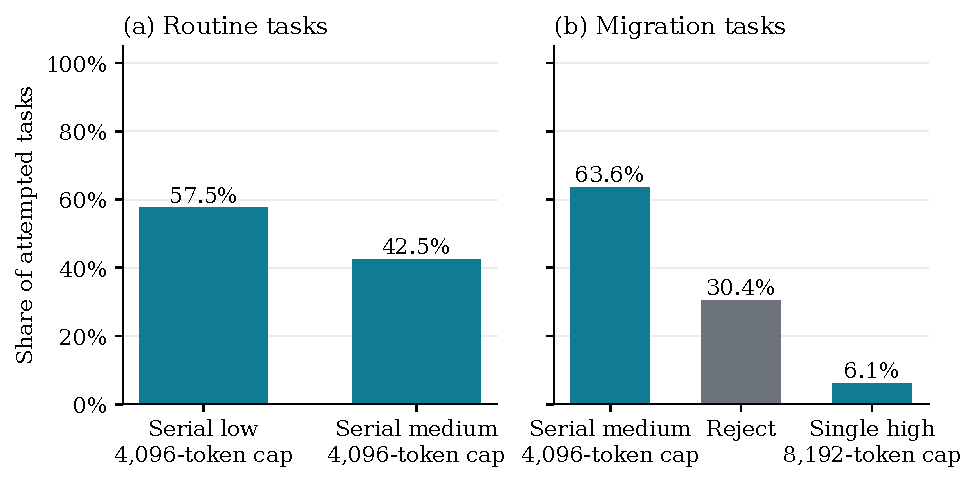
\includegraphics[width=.9\linewidth]{figures/selected-routing.pdf}
\caption{Routing weights for the exact synthetic optimum.
Bars show shares of attempted tasks, including immediate rejection.
Each label gives effort and the per-call generated-token cap.
All non-reject routes use \texttt{gemini-4-hydrogen} because the synthetic outcome and usage laws are identical across providers and its tariff is lower.
Completion is constrained across each scenario as a whole.}
\label{fig:simulation-routing}
\end{figure}

\begin{figure}[tbp]
\centering
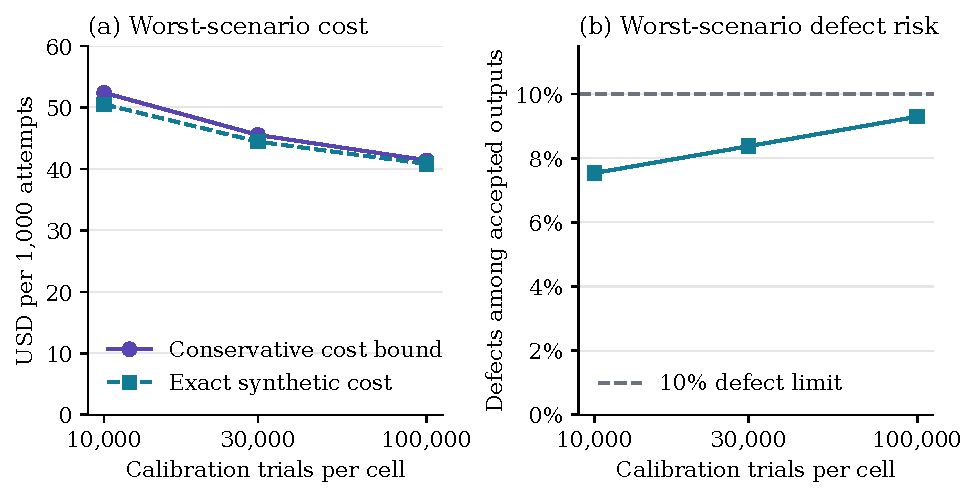
\includegraphics[width=.9\linewidth]{figures/calibration-cost-risk.pdf}
\caption{Calibration changes the selected rule.
(a) Conservative cost bound and exact synthetic population cost.
(b) Maximum accepted-defect fraction across scenarios.
Each sample size uses one independently seeded draw and a new LP solve.
Connecting lines aid comparison.
There are 216 uncertain group--candidate--scenario cells, with $\alpha=0.05$ within each experiment.
At 1,000 and 3,000 trials per cell the programme is infeasible.
Shown rules meet population acceptance and lateness constraints.
Exact enumeration supplies the evaluation values.
The five experiments have separate coverage guarantees.}
\label{fig:simulation-calibration}
\end{figure}


\section{Deployment and scope}
\label{sec:discussion}
The selector uses the same task-group rule in every scenario that the platform cannot distinguish before routing.
An observed provider-load signal can justify a richer group definition if its distribution and the corresponding cell outcomes remain valid across the permitted rules.
Queue length may depend on past routing choices, so observing it before each decision is insufficient to establish this condition.
Using an unobserved scenario label at routing time would give the optimiser information unavailable to the deployed system.
Unknown task-group proportions likewise need explicit uncertainty treatment, for example through additional justified scenario vertices.

Shared resources can make a configuration's deadline distribution depend on the routing mix.
Suppose two simultaneous tasks each select one of two services independently with equal probability.
Each service completes one task on time, while two tasks assigned to the same service both finish late.
Half of the four equally likely assignments then make both tasks late.
This gives a lateness probability of one half, although isolated executions always meet the deadline.
The selection coefficients require measurements under the intended mix, bounds valid across the permitted load range, or evaluation of complete routing and scheduling policies under their operating loads.

Suppose the scheduler bounds total added queue delay by $Q$ per attempted
workflow across the operating range. Write $T_0$ for execution time without that added delay.
Measure the tail at $d-Q$ and use $\Pr(T_0+Q>d\mid g,\theta_j,k)$ as the
lateness coefficient for a queued attempt. The event $T_0+W>d$ implies
$T_0+Q>d$ whenever actual added delay $W\le Q$.
This bound permits dependence between delay and execution time.
If the scheduler instead bounds the probability of $W>Q$ uniformly by
$\eta$ within a cell, the union bound permits adding $\eta$ to that tail, capped at one.
The other coefficients still require valid bounds when load changes behaviour.
Immediate rejection without queueing retains zero delay in the simulation.

Applying a 5\,s envelope to the existing population optimum raises its
adverse-scenario lateness bound to 15.33\%. Reoptimising restores the 15\%
bound at USD~0.0388967 per attempt. A 30\,s envelope gives USD~0.0407027.
A 50\,s envelope makes the envelope-based LP infeasible. These are sensitivity
calculations under stipulated service and delay laws.
A live pilot would need evidence for the delay bound under the permitted load.

If the service counts only outputs accepted by the deadline, use
$A'=A(1-L)$ and $Y'=Y(1-L)$ and retain lateness per attempt.
The original aggregate solution accepts only 66.56\% of adverse-scenario
attempts on time. Reoptimising at the same limits with the timely definition
costs USD~0.0477038 per attempt in the simulator.
This experiment uses its original duration distribution.
Under additional uncertain delay, the accepted population can change with
lateness, so its conditional defect risk needs its own bound.

Defect labels need a fixed criterion and reliable assessment independent of the workflow's acceptance decision.
For release notes, an omitted required migration instruction is one possible criterion.
A classifier that learns the workflow's own acceptance verdict would estimate that verdict's behaviour.
To interpret it as material correctness requires evidence connecting the verdict to the criterion.

The choice of objective also expresses an engineering preference.
Expected cost per attempt is appropriate when attempted demand defines the accounting unit.
A cost-per-accepted-output objective introduces a ratio and calls for the corresponding fractional formulation \cite{boyd}.
If every task must receive an accepted result, the completion floor is one and the fallback belongs in the complete workflow, together with its delay and cost.
An additional mean-time requirement can be expressed using calibrated bounds on $\E[T]$.
A weighted cost--time objective requires explicit normalising units and a preference weight.

An operational pilot should compare the selected rule with the current pipeline at the same service thresholds.
A strong single-model baseline tests whether additional communication earns its cost.
Run the fixed selection rule on fresh representative tasks under its expected load, counting every attempted task when assessing completion and lateness.
Development cost belongs in the decision as well.
Evaluating $N$ tasks under $J$ workflows with at most $H$ model calls each permits up to $NJH$ calls per scenario, before independent assessment.
A low-volume application can favour a smaller search even when a larger search improves per-run cost.

The graph abstraction specifies executable choices at the resolution needed for configuration search.
The finite programme then gives an optimal mix for its coefficients and candidate set.
Deployment evidence must establish how well those coefficients describe the task population and shared resources.
That evidence is the basis for deciding whether a richer search or predictor improves the engineering result.

\appendix
\FloatBarrier
\section{An exact arithmetic check}
\label{app:exact}
The small example below verifies the relation between a new graph column and the minimum cost without relying on floating-point arithmetic.
Use acceptance probabilities $(1,4/5,0,9/10)$ and nominal accepted-defect probabilities $(1/5,1/25,0,9/200)$.
Let costs be $(1,3,0,11/5)$ and lateness probabilities $(1/10,1/20,0,3/100)$.
These are stipulated complete-policy outcomes.
The adverse scenario multiplies accepted-defect probabilities by $6/5$ and leaves the other coefficients fixed.
Set completion at least $3/5$, conditional defect at most $1/10$ and lateness at most $2/25$.

The first three candidates have optimum cost $113/60$.
Their adverse-defect and completion dual multipliers can be taken as $275/18$ and $113/36$.
The fourth candidate has reduced cost $-47/40$ under that solution.
With all four candidates, weights
\begin{equation}
\left(\frac2{15},0,\frac{47}{135},\frac{14}{27}\right)
\label{eq:exact-weights}
\end{equation}
attain cost $172/135$, completion $3/5$ and worst-scenario conditional defect $1/10$.
Lateness is $13/450$.
To prove optimality, take $\beta=650/81$ and $\kappa=172/81$.
For the four candidates, the values
\begin{equation}
c_j+\beta(b_{j,\mathrm{adverse}}-a_j/10)-\kappa a_j
\label{eq:exact-slack}
\end{equation}
are $0,47/45,0,0$.
Their nonnegativity implies $c(w)\ge\kappa\gamma=172/135$ for every feasible mix.
The weights in \eqref{eq:exact-weights} attain that lower bound.
The reproduction script checks both the rational witness and the numerical solution.

\begingroup
\raggedright
\bibliographystyle{plainnat}
\bibliography{references}
\endgroup
\end{document}
